\documentclass[11pt]{style/memo}

\usepackage{tikz}
    \usetikzlibrary{arrows.meta}
\usepackage{amsmath, amssymb}
\usepackage{cancel}
\usepackage{multirow}
\usepackage{colortbl, xcolor}

\title{Parallel 2D Physics}
\author{Kevin J. Dugan}
\date{November 14, 2022}

\begin{document}
\maketitle

\section{2D Basis Functions}
Let's look at the discretization and basis functions for a 2D mesh
typical for physics simulations. We'll use quadrilateral/hexahedral
elements because they offer a direct extension from 1D elements through
tensor products. As usual, we assume that the simulation domain is
discretized using a non-overlapping set of $N$ cells $\Omega$. For a 2D
domain, we can structure the discretization as

\begin{equation*}
    \Omega = \begin{bmatrix}
        x_0 & x_1 & x_2 & x_3 \\
        x_4 & x_5 & x_6 & x_2 \\
        \vdots & \vdots & \vdots & \vdots \\
        x_{M-3} & x_{M-2} & x_{M-1} & x_M
    \end{bmatrix}
\end{equation*}

where there are $M+1$ vertices in the mesh. Note that the typical data
structure would have a level of indirection where there would be an
ordered set of spatial points, then the mesh would be defined by a
connectivity matrix where each row would reference the indices of a cell's
vertices. It should be noted here that the ordering of the vertices
should be consistent, e.g.\ in a counter-clockwise sense. We'll expand on
this concept later.


We'll start with a definition of hierarchical basis functions ($\vec{b}_i$) on a reference
element ($\mathcal{E}$).

\begin{equation}
    \label{eq:hier1d}
    \vec{b}(\xi) = \frac{1}{2} \begin{bmatrix}
        1-\xi \\
        1+\xi \\
        2 \left( 1-x^2 \right) \\
        \frac{9}{8} \left( 1 - 3\xi - \xi^2 + 3\xi^3\right)
    \end{bmatrix}
    \qquad
    \xi \in [-1,1]
\end{equation}

which are visualized in Figure~\ref{fig:hier1d}

\begin{figure}[h]
    \centering
    \begin{tikzpicture}
        \draw[gray] (-5,5) -- (5.5,5);
        \draw[gray] (5,0) -- (5,5.5);
        \draw[thick, -{>[scale=1.5]}] (-5.5,0) node[anchor=east] {0} -- (5.5,0);
        \draw[thick] (0,0.1) -- (0,-0.1) node[anchor=north] {0};
        \draw[thick] (5,0.1) -- (5,-0.1) node[anchor=north] {1};
        \draw[thick, -{>[scale=1.5]}] (-5,-0.5) node[anchor=north] {-1} -- (-5,5.5);
        \draw[thick] (-4.9,5) -- (-5.1,5) node[anchor=east] {1};

        % \draw
    \end{tikzpicture}
    \caption{Hierarchical Lagrangian basis functions up to order 3}
    \label{fig:hier1d}
\end{figure}

With a 2D reference element ($\mathcal{E}^2 = \{x,y|x,y\in \left[-1,1\right]\}$), the
2D basis functions can be defined through a tensor product of the 1D basis functions.
Note that this only applies on quadrilateral/hexahedral elements.

\begin{equation}
    \vec{b}(\xi,\eta) = \vec{b}(\xi)\vec{b}^{\, T}(\eta)
\end{equation}

Expanding the hierarchical elements defined in Equation~\ref{eq:hier1d}, only up to
quadratic order for brevity, yields the following

\begin{equation}
    \label{eq:hier2d}
    \vec{b}(\xi,\eta) = \frac{1}{4} \begin{bmatrix}
        & \cellcolor{blue!20!white} (1-\xi)(1-\eta) & \cellcolor{blue!20!white} (1-\xi)(1+\eta) & \cellcolor{red!20!white} 2(1-\xi)(1-\eta^2) \\
        & \cellcolor{blue!20!white} (1+\xi)(1-\eta) & \cellcolor{blue!20!white} (1+\xi)(1+\eta) & \cellcolor{red!20!white} 2(1+\xi)(1-\eta^2) \\
        & \cellcolor{red!20!white} 2(1-\xi^2)(1-\eta) & \cellcolor{red!20!white} 2(1-\xi^2)(1+\eta) & \cellcolor{red!20!white} 4(1-\xi^2)(1-\eta^2)
    \end{bmatrix}
\end{equation}

where regions highlighted with light blue ({\color{blue!20!white}\rule{1em}{1em}})
correspond to linear shape functions and regions highlighted with light red
({\color{red!20!white}\rule{1em}{1em}}) correspond to quadratic shape functions.

Keep in mind that the matrix structure shown in Equation~\ref{eq:hier2d} is only for
illustrative purposes; all the basis functions defined are used as an unordered set of
functions during matrix assembly for example.

We've based this discussion on functions defined on a reference element, which means
that during the system construction we'll need to map the physical element to the
reference element. We'll stipulate that the physical elements need to have straight
edges so that a bilinear map can be used for the transformation --- curved elements
would require a higher order map for the transformation.

Coincidentally, the bilinear map for the transformation can be constructed from the
linear basis functions shown in Equation~\ref{eq:hier2d}. The 1D transformation is
defined as

\begin{equation}
    x = b_0(\xi) x_L + b_1(\xi) x_R
\end{equation}

Similarly, the 2D bilinear transformation can be constructed using the tensor product
of linear basis functions. We impose a column-wise ordering on the basis functions
which corresponds to a counter-clockwise ordering of the element vertices. We'll define
the 2D transformation taking advantage of the Einstein summation notation

\begin{eqnarray}
    \begin{bmatrix}
        x & y
    \end{bmatrix} = \frac{1}{4}
    \begin{bmatrix}
        (1-\xi)(1-\eta) \\
        (1+\xi)(1-\eta) \\
        (1-\xi)(1+\eta) \\
        (1+\xi)(1+\eta)
    \end{bmatrix}^T
    \begin{bmatrix}
        x_0 & y_0 \\
        x_1 & y_1 \\
        x_2 & y_2 \\
        x_3 & y_3
    \end{bmatrix}
    = \frac{1}{4}
    \begin{bmatrix}
        \vec{b}_i(\xi,\eta)x^i &
        \vec{b}_i(\xi,\eta)y^i
    \end{bmatrix}
\end{eqnarray}

The Jacobian $\mathcal{J}$ for element $e$ can be defined in the following way

\begin{equation*}
    \mathrm{1D:} \quad \mathcal{J}_e = \frac{dx}{d\xi} = \frac{db_i}{d\xi}x_i = \frac{db_0}{d\xi}x_L + \frac{db_1}{d\xi}x_R
\end{equation*}
\begin{equation*}
    \mathrm{2D:} \quad \mathcal{J}_e = \begin{bmatrix}
        \frac{\partial b_i}{\partial\xi}x_i & \frac{\partial b_i}{\partial\xi}y_i \\
        \frac{\partial b_i}{\partial\eta}x_i & \frac{\partial b_i}{\partial\eta}y_i
    \end{bmatrix}
\end{equation*}

In general, the Jacobian matrix will be defined from the following relation

\begin{equation*}
    \mathcal{J}_e = \begin{bmatrix}
        \frac{\partial x}{\partial\xi} & \frac{\partial y}{\partial\xi} & \frac{\partial z}{\partial\xi} \\
        \frac{\partial x}{\partial\eta} & \frac{\partial y}{\partial\eta} & \frac{\partial z}{\partial\eta} \\
        \frac{\partial x}{\partial\omega} & \frac{\partial y}{\partial\omega} & \frac{\partial z}{\partial\omega}
    \end{bmatrix}
\end{equation*}

We can visualize the transformation of a 2D element in Figure~\ref{fig:transform2d}.

\begin{figure}[h]
\centering
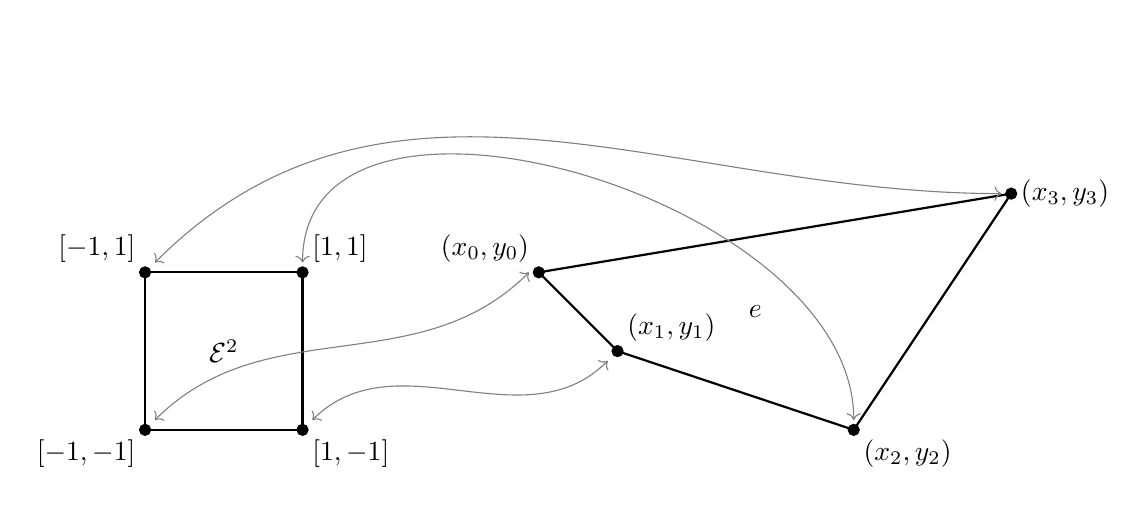
\begin{tikzpicture}[scale=2]
    % Reference Element
    \draw[thick] (0,0) -- (1,0) -- (1,1) -- (0,1) -- (0,0);
    \node at (0.5, 0.5) {$\mathcal{E}^2$};
    % Lower Left
    \draw[fill] (0,0) circle [radius=1pt];
    \node (A) at (0,0) {};
    \node[below left] at (0,0) {$[-1,-1]$};
    % Lower Right
    \draw[fill] (1,0) circle [radius=1pt];
    \node (B) at (1,0) {};
    \node[below right] at (1,0) {$[1,-1]$};
    % Upper Right
    \draw[fill] (1,1) circle [radius=1pt];
    \node (C) at (1,1) {};
    \node[above right] at (1,1) {$[1,1]$};
    % Upper Left
    \draw[fill] (0,1) circle [radius=1pt];
    \node (D) at (0,1) {};
    \node[above left] at (0,1) {$[-1,1]$};

    % Distorted Element
    \draw[thick] (3,0.5) -- (4.5,0) -- (5.5,1.5) -- (2.5,1) -- (3,0.5);
    \node at (3.875,0.75) {$e$};
    % Lower Left
    \draw[fill] (3,0.5) circle [radius=1pt];
    \node (X) at (3,0.5) {};
    \node[above right] at (3,0.5) {$(x_1,y_1)$};
    % Lower Right
    \draw[fill] (4.5,0) circle [radius=1pt];
    \node (Y) at (4.5,0) {};
    \node[below right] at (4.5,0) {$(x_2,y_2)$};
    % Upper Right
    \draw[fill] (5.5,1.5) circle [radius=1pt];
    \node (Z) at (5.5,1.5) {};
    \node[right] at (5.5,1.5) {$(x_3,y_3)$};
    % Lower Left
    \draw[fill] (2.5,1) circle [radius=1pt];
    \node (W) at (2.5,1) {};
    \node[above left] at (2.5,1) {$(x_0,y_0)$};

    % Mapping lines
    \draw[<->, gray] (A.north east) [out=45,in=225] to (W.west);
    \draw[<->, gray] (B.north east) [out=45,in=225] to (X.south west);
    \draw[<->, gray] (C.north)      [out=90,in=90]  to (Y.north);
    \draw[<->, gray] (D.north east) [out=45,in=180] to (Z.west);

\end{tikzpicture}
\caption{Transformation between mesh element and reference element}
\label{fig:transform2d}
\end{figure}

\nocite{segerlind-1984, zienkiewicz-2005, guermond-2000}
\bibliographystyle{unsrt}
\bibliography{references}

\end{document}